\documentclass{article}
\usepackage{graphicx}
\usepackage{amsthm}
\usepackage{amssymb}
\usepackage{amsmath}
\usepackage{parskip}
\usepackage[margin=0.6in]{geometry}
\usepackage{tikz}
\usepackage{titling}

 % move title upward

\title{15.095 Machine Learning HW1}
\author{Chris Low}
\date{} % removes the date

\begin{document}

\maketitle

\section*{Question 1}

\subsection*{(a)}

\textbf{False.}

\noindent First, the primal is infeasible. The first two constraints imply


\[
x \leq y
\]
and
\[
-x+y\leq -1
\quad\Longrightarrow\quad
y\leq x-1.
\]

\noindent Any feasible solution would have to satisfy
\[
x\leq y\leq x-1,
\]
which is impossible. Hence, the primal is infeasible.

\vspace{3mm}

\noindent To determine whether the dual is unbounded, we can rewrite the primal constraints as
\[
x-y\leq 0,
\]
\[
-x+y\leq -1.
\]

\noindent Using the dual variables $u_1,u_2\geq 0$ and the equation, the dual is
\[
\min \quad -u_2
\]
subject to
\[
u_1-u_2\geq 1,
\]
\[
-u_1+u_2\geq 2,
\]
\[
u_1,u_2\geq 0.
\]

\noindent If both constraints must be true, their sum must also be true.

\[
(u_1-u_2)+(-u_1+u_2)\geq 1+2,
\]
so
\[
0\geq 3,
\]
which is impossible. So, the dual is \textbf{infeasible}, not unbounded. The statement is false. \qed

\newpage

\subsection*{(b)}
\textbf{False.}

\noindent From lecture, for a Frobenius norm uncertainty set,

\[
\mathcal{U}_{F(q)}
=
\left\{
\Delta \in \mathbb{R}^{n \times p}
:
\|\Delta\|_{q-F} \leq \rho
\right\},
\]
where
\[
\|\Delta\|_{q-F}
=
\left(
\sum_{i,j} |\Delta_{ij}|^q
\right)^{1/q},
\]

\noindent we get the equivalence of robustness and regularization as

\[
\min_{\beta}
\max_{\Delta \in \mathcal{U}_{F(q)}}
\|y-(X+\Delta)\beta\|_q
=
\min_{\beta}
\|y-X\beta\|_q
+
\rho\|\beta\|_{q^*},
\]
where
\[
\frac{1}{q}+\frac{1}{q^*}=1.
\]

\noindent We take \(q=2\), and we have \(q^*=2\), so
\[
\min_{\beta}
\max_{\Delta:\|\Delta\|_{2-F}\leq\mu}
\|y-(X+\Delta)\beta\|_2
=
\min_{\beta}
\|y-X\beta\|_2
+
\mu\|\beta\|_2.
\]


\[
\|\Delta\|_{2-F}
=
\left(
\sum_{i,j}\Delta_{ij}^2
\right)^{1/2},
\]
Since this places one bound on the perturbation across the \textbf{entire} matrix \(X\), this corresponds to a \emph{global}
perturbation. Therefore,
\[
\mu\|\beta\|_2
\quad\text{is a global perturbation bounded by }\mu.
\]

\noindent For an induced norm uncertainty set,
\[
\mathcal{U}_{(r,q)}
=
\left\{
\Delta \in \mathbb{R}^{n \times p}
:
\|\Delta\|_{r,q}\leq\rho
\right\},
\]


\[
\|\Delta\|_{r,q}
=
\max_x
\frac{\|\Delta x\|_q}{\|x\|_r},
\]

\noindent we have the theorem 
\[
\min_{\beta}
\max_{\Delta\in\mathcal{U}_{(r,q)}}
\|y-(X+\Delta)\beta\|_q
=
\min_{\beta}
\|y-X\beta\|_q
+
\rho\|\beta\|_r.
\]

\noindent Let \(r=1\), \(q=2\), and \(\rho=\lambda\),
\[
\min_{\beta}
\max_{\Delta:\|\Delta\|_{1,2}\leq\lambda}
\|y-(X+\Delta)\beta\|_2
=
\min_{\beta}
\|y-X\beta\|_2
+
\lambda\|\beta\|_1.
\]

\noindent The induced \((1,2)\)-norm uncertainty set
matches with \emph{feature-wise} perturbations. Therefore,
$\lambda\|\beta\|_1$ corresponds to feature-wise perturbations bounded by $\lambda$.

\vspace{3mm}

\noindent So, for the Elastic Net objective
\[
\min_{\beta}
\|y-X\beta\|_2
+
\lambda\|\beta\|_1
+
\mu\|\beta\|_2,
\]


$\lambda$ corresponds to feature-wise perturbations, and $\mu$ corresponds to global perturbations. \qed


\vspace{7mm}

\subsection*{(c)}
\textbf{True.}

\vspace{3mm}



\noindent 1. The objective
\[
\min_{x,y} \|x-y\|_1
=
\min_{x,y} \sum_{i=1}^n |x_i-y_i|.
\]

Introduce variables $t_i \geq 0$, 
\[
\boxed{t_i \geq x_i-y_i,\quad t_i \geq -(x_i-y_i),\quad i=1,\ldots,n.}
\]

Since we are minimizing $\sum_i t_i$ and $t_i \geq 0$, this implies
\[
t_i=|x_i-y_i|.
\]

So, we have our objective: 
\[
\min \sum_{i=1}^n t_i.
\]

2. 
\[
\|x\|_1+\|y\|_1\geq 2.
\]

Write each variable with its positive and negative
parts:
\[
x_i=x_i^+-x_i^-,
\]
\[
y_i=y_i^+-y_i^-,
\]
where
\[
x_i^+,x_i^-,y_i^+,y_i^- \geq 0.
\]

Introduce binary variables $s_i,r_i\in\{0,1\}$ with the conditions:
\[
x_i^+ \leq Ms_i,
\]
\[
x_i^- \leq M(1-s_i),
\]
\[
y_i^+ \leq Mr_i,
\]
\[
y_i^- \leq M(1-r_i).
\]

This ensures that at most one of the positive and negative
parts is nonzero. Therefore,
\[
|x_i|=x_i^++x_i^-,
\]
and
\[
|y_i|=y_i^++y_i^-.
\]

Hence,
\[
\|x\|_1+\|y\|_1\geq 2
\]
becomes
\[
\boxed{
\sum_{i=1}^n
\left(
x_i^+ + x_i^- + y_i^+ + y_i^-
\right)
\geq 2.}
\]


3. 
\[
\|y\|_0\leq 5.
\]

Let $z_i\in\{0,1\}$ and impose
\[
\boxed{
-Mz_i\leq y_i\leq Mz_i,
\qquad i=1,\ldots,n,}
\]
and
\[
\boxed{
\sum_{i=1}^n z_i\leq 5.}
\]

If $z_i=0$, then $y_i=0$. Thus, at most five components of $y$
can be nonzero.

\vspace{3mm}

4. 


\[
\|x\|_\infty\leq M
\]
is equivalent to
\[
\boxed{
-M\leq x_i\leq M,
\qquad i=1,\ldots,n,}
\]
and
\[
\|y\|_\infty\leq M
\]
is equivalent to
\[
\boxed{
-M\leq y_i\leq M,
\qquad i=1,\ldots,n.}
\]

All parts of the problem can be represented using linear
constraints and/or binary variables, so the problem can be reformulated
as a mixed-integer linear optimization problem. \qed



\subsection*{(d)}
\textbf{False.}

Let
\[
r = y-X\beta.
\]

The inner maximization: 
\[
\max_{\|\delta\|_2\leq\lambda}\|r+\delta\|_2.
\]

By the triangle inequality,
\[
\|r+\delta\|_2
\leq
\|r\|_2+\|\delta\|_2.
\]

Since
\[
\|\delta\|_2\leq\lambda,
\]

\[
\|r+\delta\|_2
\leq
\|r\|_2+\lambda.
\]

This upper bound can be achieved by (for $r\neq 0$)
\[
\delta
=
\lambda\frac{r}{\|r\|_2}.
\]

This choice uses the full budget $\|\delta\|_2=\lambda$ and points $\delta$ in the same direction as $r$, so it increases the residual norm as much as possible.

Since $\delta$ points in the same direction as $r$, the triangle
inequality can proceed with equality: 
\[
\begin{aligned}
\|r+\delta\|_2
&=
\left\|
r+\lambda\frac{r}{\|r\|_2}
\right\|_2 \\
&=
\left\|
\left(1+\frac{\lambda}{\|r\|_2}\right)r
\right\|_2 \\
&=
\left(1+\frac{\lambda}{\|r\|_2}\right)\|r\|_2 \\
&=
\|r\|_2+\lambda.
\end{aligned}
\]


Hence,
\[
\max_{\|\delta\|_2\leq\lambda}
\|y+\delta-X\beta\|_2
=
\|y-X\beta\|_2+\lambda.
\]

The robust optimization problem is
\[
\boxed{
\min_\beta
\left(
\|y-X\beta\|_2+\lambda
\right)}
\]
not
\[
\min_\beta
\left(
\|y-X\beta\|_2+\lambda\|\beta\|_2
\right).
\]

\qed



\subsection*{(e)}
\textbf{False.}

The cutting-plane algorithm is not run directly on the big-$M$
formulation. The big-$M$ formulation keeps the regression coefficients
$\beta$ and uses binary variables $z_j$ to determine which coefficients
can be nonzero.

Instead, Theorem 3.2 rewrites the problem as
\[
\min_{s\in S_k^p}
\frac{1}{2}y^T
\left(
I_n+\gamma\sum_{j\in[p]}s_jK_j
\right)^{-1}y,
\]
where
\[
K_j=X_jX_j^T
\]
and $s_j=1$ if feature $j$ is selected and $s_j=0$ otherwise. 

This
removes $\beta$ from the optimization and does not require big-$M$
constraints.

If we call the objective $c(s)$, the problem is simply
\[
\min_{s\in S_k^p} c(s).
\]
Since $c(s)$ is convex, the cutting-plane algorithm approximates it using
linear cuts
\[
\eta \geq c(s_i)+\nabla c(s_i)^T(s-s_i),
\]
where $s_i$ is the feature selection found at iteration $i$. More cuts
are added as the algorithm runs, and this gives us a better approximation of
$c(s)$.

Therefore, the cutting-plane algorithm is run on the formulation from
Theorem 3.2, not directly on the big-$M$ formulation. \qed 

\subsection*{(f)}

\textbf{True.}

Lasso solves
\[
\min_\beta \|y-X\beta\|_2+\lambda\|\beta\|_1,
\]
where
\[
\|\beta\|_1=\sum_{j=1}^p |\beta_j|.
\]

The $\ell_1$ penalty penalizes the magnitude of the regression
coefficients. As $\lambda$ increases, the coefficients are pushed toward
zero, and some may become exactly zero. Therefore, Lasso encourages
sparsity and can effectively remove features from the model.

Sparse regression, however, directly imposes a constraint on the number
of nonzero coefficients, such as
\[
\|\beta\|_0 \leq k.
\]

For example, if $k=2$, sparse regression guarantees that at most two
coefficients are nonzero. Lasso may still have more than two nonzero
coefficients depending on the value of $\lambda$.

Thus, Lasso encourages sparsity through an $\ell_1$ penalty, while sparse
regression explicitly restricts the number of selected features. The two
problems are therefore not equivalent in general.


\newpage

\section*{Question 2}
\subsection*{Part A}

\subsection*{(a.)}

By definition of the induced norm,
\[
\|\Delta\|_{(\infty,\infty)}
=
\max_{x\neq 0}
\frac{\|\Delta x\|_\infty}{\|x\|_\infty}.
\]

For any $x\neq 0$, define
\[
\tilde{x}=\frac{x}{\|x\|_\infty},
\]
so that $\|\tilde{x}\|_\infty=1$. Since
$x=\|x\|_\infty\tilde{x}$, we have
\[
\frac{\|\Delta x\|_\infty}{\|x\|_\infty}
=
\frac{\|\Delta(\|x\|_\infty\tilde{x})\|_\infty}
{\|x\|_\infty}
=
\|\Delta\tilde{x}\|_\infty.
\]

Thus, it is sufficient to maximize over vectors with
$\|x\|_\infty=1$, giving
\[
\|\Delta\|_{(\infty,\infty)}
=
\max_{\|x\|_\infty=1}\|\Delta x\|_\infty.
\]

Let $\delta_i^T$ denote each row $i$ of $\Delta$. Then
\[
\Delta x
=
\begin{pmatrix}
\delta_1^T x\\
\vdots\\
\delta_n^T x
\end{pmatrix},
\]


\[
\|\Delta x\|_\infty
=
\max_{i\in[n]}|\delta_i^T x|.
\]


\[
\|\Delta\|_{(\infty,\infty)}
=
\max_{\|x\|_\infty=1}
\max_{i\in[n]}|\delta_i^T x|.
\]

Since both operations are maximizations (hint (i)), their order can be exchanged:
\[
\|\Delta\|_{(\infty,\infty)}
=
\max_{i\in[n]}
\max_{\|x\|_\infty=1}
|\delta_i^T x|.
\]

\vspace{5mm}
Moving onto hint (ii.), we need to show upper and lower bound can be established. We now show that, for each row $i$,
\[
\max_{\|x\|_\infty=1}|\delta_i^T x|
=
\|\delta_i\|_1.
\]

For any $x$ satisfying $\|x\|_\infty=1$, we can expand
$\delta_i^T x$ as a dot product:
\[
\delta_i^T x
=
\sum_{j=1}^p \delta_{ij}x_j.
\]

We then apply the triangle inequality and take absolute values: 
\[
|\delta_i^T x|
=
\left|
\sum_{j=1}^p \delta_{ij}x_j
\right|
\leq
\sum_{j=1}^p |\delta_{ij}x_j|
=
\sum_{j=1}^p |\delta_{ij}||x_j|.
\]


Since $\|x\|_\infty=1$, we have $|x_j|\leq 1$ for every $j$.
Thus,
\[
|\delta_i^T x|
\leq
\sum_{j=1}^p |\delta_{ij}||x_j|
\leq
\sum_{j=1}^p|\delta_{ij}|
=
\|\delta_i\|_1.
\]

Therefore,
\[
\max_{\|x\|_\infty=1}|\delta_i^T x|
\leq
\|\delta_i\|_1.
\]

\vspace{5mm}
For the reverse inequality lower bound, choose
\[
x_j=\operatorname{sign}(\delta_{ij}).
\]
This choice satisfies $\|x\|_\infty=1$, and
\[
\delta_i^T x
=
\sum_{j=1}^p
\delta_{ij}\operatorname{sign}(\delta_{ij})
=
\sum_{j=1}^p|\delta_{ij}|
=
\|\delta_i\|_1.
\]

So we have, 
\[
\max_{\|x\|_\infty=1}|\delta_i^T x|
\geq
\|\delta_i\|_1.
\]

Combine the two inequalities: 
\[
\max_{\|x\|_\infty=1}|\delta_i^T x|
=
\|\delta_i\|_1.
\]

Substituting this back into the induced norm gives
\[
\|\Delta\|_{(\infty,\infty)}
=
\max_{i\in[n]}\|\delta_i\|_1.
\] \qed

\vspace{5mm}

The switch from $1$ to $\infty$ comes from the dual-norm relationship
between $\ell_1$ and $\ell_\infty$. In particular, as shown above,
\[
\max_{\|x\|_\infty=1} |\delta_i^T x|
=
\|\delta_i\|_1.
\]
Thus, if we constrain $x$ using the $\ell_\infty$ norm, we produce the
$\ell_1$ norm of the row $\delta_i$. This is because $\ell_1$ and
$\ell_\infty$ are dual norms, so this explains why an $\ell_1$ row budget
corresponds to a first induced-norm index of $\infty$.

\vspace{5mm}
If instead the row budget were
\[
\|\delta_i\|_2 \leq \rho
\qquad \text{for all } i,
\]
then the first induced-norm index would be $2$.

From the definition of the induced norm, we consider
\[
\|\Delta\|_{(2,\infty)}
=
\max_{x\neq 0}
\frac{\|\Delta x\|_\infty}{\|x\|_2}.
\]
Since scaling $x$ does not change this ratio, we can normalize $x$ by
dividing it by $\|x\|_2$. Therefore, it is sufficient to consider
vectors satisfying
\[
\|x\|_2=1.
\]

For each row $\delta_i$, by the Cauchy--Schwarz inequality,
\[
|\delta_i^T x|
\leq
\|\delta_i\|_2\|x\|_2.
\]
Since $\|x\|_2=1$, this gives
\[
|\delta_i^T x|
\leq
\|\delta_i\|_2.
\]
Therefore,
\[
\max_{\|x\|_2=1}|\delta_i^T x|
\leq
\|\delta_i\|_2.
\]

To show that this upper bound can be attained, choose
\[
x=\frac{\delta_i}{\|\delta_i\|_2}.
\]
This is a valid choice because
\[
\|x\|_2
=
\left\|
\frac{\delta_i}{\|\delta_i\|_2}
\right\|_2
=
\frac{\|\delta_i\|_2}{\|\delta_i\|_2}
=
1.
\]


\[
|\delta_i^T x|
=
\left|
\delta_i^T
\frac{\delta_i}{\|\delta_i\|_2}
\right|
=
\frac{\delta_i^T\delta_i}{\|\delta_i\|_2}.
\]
Since
\[
\delta_i^T\delta_i=\|\delta_i\|_2^2,
\]


\[
|\delta_i^T x|
=
\frac{\|\delta_i\|_2^2}{\|\delta_i\|_2}
=
\|\delta_i\|_2.
\]
Thus,
\[
\max_{\|x\|_2=1}|\delta_i^T x|
\geq
\|\delta_i\|_2.
\]

Combining the upper and lower bounds gives
\[
\max_{\|x\|_2=1}|\delta_i^T x|
=
\|\delta_i\|_2.
\]

Thus, $\ell_2$ is self-dual, corresponding to a first induced-norm index of $2$. 

Therefore, an $\ell_2$ constraint on $x$ produces the $\ell_2$ norm of
each row $\delta_i$, so the first induced-norm index is $2$. The second
index remains $\infty$ because $\|\Delta x\|_\infty$ takes the maximum
over the rows. Thus, the corresponding uncertainty set is
\[
\mathcal{U}_{(2,\infty)}.
\]

\vspace{7mm}

\subsection*{(b.)}


For $n=1$ and $p=2$, the perturbation matrix consists of a single row, so each possible perturbation can be represented as a point in the 
$(\Delta_{11},\Delta_{12})$ plane.
\[
\delta_1=(\Delta_{11},\Delta_{12})\in\mathbb{R}^2.
\]


For $\mathcal A$, since there is only one row,
\[
\|\Delta_j\|_\infty \leq \lambda
\]
\[
|\Delta_{11}|\leq\lambda,
\qquad
|\Delta_{12}|\leq\lambda.
\]
\[
\mathcal A
=
\left\{
(\Delta_{11},\Delta_{12}):
|\Delta_{11}|\leq\lambda,\;
|\Delta_{12}|\leq\lambda
\right\},
\]
which is a square centered at the origin with corners
$(\pm\lambda,\pm\lambda)$.

For $\mathcal B$, 
\[
\|\delta_1\|_1\leq\rho,
\]
\[
|\Delta_{11}|+|\Delta_{12}|\leq\rho.
\]
\[
\mathcal B
=
\left\{
(\Delta_{11},\Delta_{12}):
|\Delta_{11}|+|\Delta_{12}|\leq\rho
\right\},
\]
which is a diamond centered at the origin with vertices
\[
(\rho,0),\quad(-\rho,0),\quad(0,\rho),\quad(0,-\rho).
\]

The three possible cases are shown below.

\begin{center}
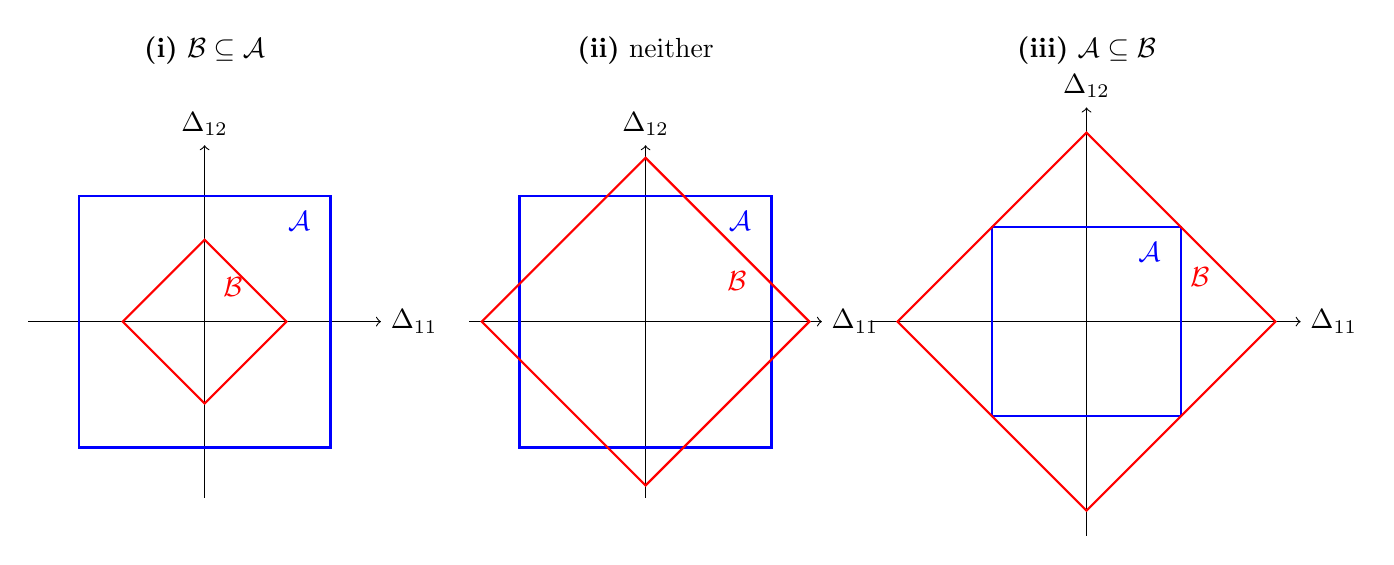
\begin{tikzpicture}[scale=0.8]

% CASE 1
\begin{scope}[xshift=0cm]
    \node at (0,4.3) {\textbf{(i)} $\mathcal B\subseteq\mathcal A$};

    % axes
    \draw[->] (-2.8,0) -- (2.8,0)
        node[right] {$\Delta_{11}$};
    \draw[->] (0,-2.8) -- (0,2.8)
        node[above] {$\Delta_{12}$};

    % A square
    \draw[blue, thick] (-2,-2) rectangle (2,2);
    \node[blue] at (1.5,1.6) {$\mathcal A$};

    % B diamond
    \draw[red, thick]
        (0,1.3) -- (1.3,0) -- (0,-1.3) -- (-1.3,0) -- cycle;
    \node[red] at (0.45,0.55) {$\mathcal B$};
\end{scope}


% CASE 2
\begin{scope}[xshift=7cm]
    \node at (0,4.3) {\textbf{(ii)} neither};

    % axes
    \draw[->] (-2.8,0) -- (2.8,0)
        node[right] {$\Delta_{11}$};
    \draw[->] (0,-2.8) -- (0,2.8)
        node[above] {$\Delta_{12}$};

    % A square
    \draw[blue, thick] (-2,-2) rectangle (2,2);
    \node[blue] at (1.5,1.6) {$\mathcal A$};

    % B diamond
    \draw[red, thick]
        (0,2.6) -- (2.6,0) -- (0,-2.6) -- (-2.6,0) -- cycle;
    \node[red] at (1.45,0.65) {$\mathcal B$};
\end{scope}


% CASE 3
\begin{scope}[xshift=14cm]
    \node at (0,4.3) {\textbf{(iii)} $\mathcal A\subseteq\mathcal B$};

    % axes
    \draw[->] (-3.4,0) -- (3.4,0)
        node[right] {$\Delta_{11}$};
    \draw[->] (0,-3.4) -- (0,3.4)
        node[above] {$\Delta_{12}$};

    % A square
    \draw[blue, thick] (-1.5,-1.5) rectangle (1.5,1.5);
    \node[blue] at (1.0,1.1) {$\mathcal A$};

    % B diamond
    \draw[red, thick]
        (0,3) -- (3,0) -- (0,-3) -- (-3,0) -- cycle;
    \node[red] at (1.8,0.7) {$\mathcal B$};
\end{scope}

\end{tikzpicture}
\end{center}

For case (i), $\mathcal B\subseteq\mathcal A$, the diamond must fit
entirely inside the square. The vertices of $\mathcal B$ extend a
distance $\rho$ along each coordinate axis, while $\mathcal A$ extends
a distance $\lambda$. Thus,
\[
\boxed{\rho\leq\lambda}.
\]

For case (ii), neither set is contained in the other. If
$\rho>\lambda$, the vertices $(\rho,0)$ and $(0,\rho)$ of $\mathcal B$
extend outside $\mathcal A$, so
\[
\mathcal B\not\subseteq\mathcal A.
\]
However, the corner $(\lambda,\lambda)$ of $\mathcal A$ has
$\ell_1$ norm
\[
|\lambda|+|\lambda|=2\lambda.
\]
If $\rho<2\lambda$, this corner does not belong to $\mathcal B$, so
\[
\mathcal A\not\subseteq\mathcal B.
\]
Therefore, neither set contains the other when
\[
\boxed{\lambda<\rho<2\lambda}.
\]


For case (iii), $\mathcal A\subseteq\mathcal B$, the diamond must be
large enough to contain all four corners of the square. At a corner,
for example $(\lambda,\lambda)$,
\[
|\Delta_{11}|+|\Delta_{12}|
=
|\lambda|+|\lambda|
=
2\lambda.
\]
Thus, all of $\mathcal A$ is contained in $\mathcal B$ when
\[
\boxed{\rho\geq2\lambda}.
\]




\vspace{7mm}
\subsection*{(c.)}


For $n=1$ and a general number of features $p$, the perturbation is
\[
\delta_1=(\Delta_{11},\ldots,\Delta_{1p})\in\mathbb{R}^p.
\]
The two sets are
\[
\mathcal A
=
\{\delta_1:\|\delta_1\|_\infty\leq\lambda\},
\qquad
\mathcal B
=
\{\delta_1:\|\delta_1\|_1\leq\rho\}.
\]


For case (i), we want $\mathcal B\subseteq\mathcal A$. If
$\delta_1\in\mathcal B$, then
\[
\|\delta_1\|_1\leq\rho.
\]
The largest individual coordinate cannot exceed the sum of the absolute
values of all coordinates: 
\[
\|\delta_1\|_\infty
\leq
\|\delta_1\|_1
\leq
\rho.
\]
Therefore, if
\[
\rho\leq\lambda,
\]
then $\|\delta_1\|_\infty\leq\lambda$, so $\delta_1\in\mathcal A$.
Hence,
\[
\boxed{
\mathcal B\subseteq\mathcal A
\quad\Longleftrightarrow\quad
\rho\leq\lambda.
}
\]

This condition is unchanged as $p$ grows because the total $\ell_1$
budget remains $\rho$, so no individual perturbation can exceed $\rho$.


\vspace{5mm}
For case (iii), we want $\mathcal A\subseteq\mathcal B$.
Since $\mathcal A$ allows each of the $p$ coordinates to have magnitude
up to $\lambda$, the largest possible $\ell_1$ norm in $\mathcal A$ is
\[
\lambda+\cdots+\lambda=p\lambda.
\]
For example, this value is attained at the corner 
\[
\delta_1=(\lambda,\ldots,\lambda).
\]
Therefore, for $\mathcal B$ to contain every point in $\mathcal A$, its
$\ell_1$ budget must satisfy
\[
\rho\geq p\lambda.
\]
Hence,
\[
\boxed{
\mathcal A\subseteq\mathcal B
\quad\Longleftrightarrow\quad
\rho\geq p\lambda.}
\]

Unlike case (i), this condition grows with $p$ because each additional
feature can contribute up to $\lambda$ to the total $\ell_1$ error.


\vspace{5mm}

For completeness, between these two cases,
\[
\boxed{
\lambda<\rho<p\lambda,
}
\]
neither set contains the other. In this range, $\mathcal B$ can extend
outside $\mathcal A$ by placing its budget on one coordinate, while the
corners $(\pm\lambda,\ldots,\pm\lambda)$ of $\mathcal A$ lie outside
$\mathcal B$. Thus, the ``neither'' range becomes wider as $p$ grows.



\newpage

\subsection*{Part B}


From Part A, we have
\[
\mathcal A=\mathcal U_{(1,\infty)}
\]
with radius $\lambda$, and
\[
\mathcal B=\mathcal U_{(\infty,\infty)}
\]
with radius $\rho$.

With the robust optimization result: 
\[
\max_{\Delta\in\mathcal A,\;\Delta'\in\mathcal B}
\left\|
y-(X+\Delta+\Delta')\beta
\right\|_\infty
=
\|y-X\beta\|_\infty
+
\lambda\|\beta\|_1
+
\rho\|\beta\|_\infty.
\]

Therefore, the original problem is equivalent to
\[
\min_\beta
\quad
\|y-X\beta\|_\infty
+
\lambda\|\beta\|_1
+
\rho\|\beta\|_\infty
\]
subject to
\[
\|\beta\|_0\leq k.
\]



\medskip
\textbf{1. $\|y-X\beta\|_\infty$}

$t\geq 0$ to represent $y_i-X_i\beta$. For each observation $i=1,\ldots,n$, 
\[
y_i-X_i\beta\leq t,
\]
\[
-(y_i-X_i\beta)\leq t.
\]

Which imply 
\[
|y_i-X_i\beta|\leq t
\qquad \forall i,
\]

Since $t$ is minimized in the objective, it will equal the largest
absolute residual:
\[
t=\|y-X\beta\|_\infty.
\]

\medskip
\textbf{2. $\lambda\|\beta\|_1$}


\[
\|\beta\|_1
=
\sum_{j=1}^p|\beta_j|,
\]
let $u_j\geq 0$ for $j=1,\ldots,p$ and impose
\[
u_j\geq\beta_j,
\]
\[
u_j\geq-\beta_j.
\]

Thus,
\[
u_j\geq|\beta_j|.
\]
Since the objective minimizes $\sum_{j=1}^p u_j$, at optimality
\[
u_j=|\beta_j|,
\]

\[
\sum_{j=1}^p u_j=\|\beta\|_1.
\]

The $\ell_1$ penalty becomes
\[
\lambda\sum_{j=1}^p u_j.
\]

\medskip
\textbf{3. $\rho\|\beta\|_\infty$}

Let $v\geq 0$ represent the largest
absolute coefficient. For each $j=1,\ldots,p$, impose
\[
-v\leq\beta_j\leq v.
\]

Therefore,
\[
|\beta_j|\leq v
\qquad \forall j.
\]
Since the objective minimizes $v$, at optimality
\[
v=\max_j|\beta_j|
=
\|\beta\|_\infty.
\]

The $\ell_\infty$ penalty becomes
\[
\rho v.
\]

\medskip
\textbf{4. $\|\beta\|_0\leq k$}

Introduce binary variables
\[
z_j\in\{0,1\},
\qquad j=1,\ldots,p,
\]
where $z_j=1$ allows feature $j$ to be selected and $z_j=0$ forces its
coefficient to zero.

Using the given big-$M$ constants $M_j$, impose
\[
-M_jz_j\leq\beta_j\leq M_jz_j
\qquad j=1,\ldots,p.
\]

If $z_j=0$, then $\beta_j=0$. If $z_j=1$, then $\beta_j$ may take any
value between $-M_j$ and $M_j$.

To allow at most $k$ nonzero coefficients, impose
\[
\sum_{j=1}^p z_j\leq k.
\]

\medskip

Putting all of the above together gives
\[
\boxed{
\min_{\beta,t,u,v,z}
\quad
t
+
\lambda\sum_{j=1}^p u_j
+
\rho v}
\]

subject to
\[
y_i-X_i\beta\leq t,
\qquad i=1,\ldots,n,
\]
\[
-(y_i-X_i\beta)\leq t,
\qquad i=1,\ldots,n,
\]
\[
u_j\geq\beta_j,
\qquad j=1,\ldots,p,
\]
\[
u_j\geq-\beta_j,
\qquad j=1,\ldots,p,
\]
\[
-v\leq\beta_j\leq v,
\qquad j=1,\ldots,p,
\]
\[
-M_jz_j\leq\beta_j\leq M_jz_j,
\qquad j=1,\ldots,p,
\]
\[
\sum_{j=1}^p z_j\leq k,
\]
\[
z_j\in\{0,1\},
\qquad j=1,\ldots,p,
\]
\[
t\geq0,\qquad
u_j\geq0,\qquad
v\geq0.
\]

($\beta_j$ is the regression coefficient for feature $j$,
$t$ represents $\|y-X\beta\|_\infty$, $u_j$ represents
$|\beta_j|$, $v$ represents $\|\beta\|_\infty$, and $z_j$ indicates
whether feature $j$ is selected.)


\end{document}